\documentclass[12pt]{amsart}
\usepackage{style}

\author{Blake Farman}
\address{Lafayette College}
\title[Review]{Final Exam Review\\Math 161}
\date{December 13, 2018}

\begin{document}
\maketitle

\theoremstyle{definition}
\newtheorem{thm}{}
\renewcommand{\qedsymbol}{}

\section*{Fill In the Blank}

\begin{thm}[6 Points - Limit Laws]
  Suppose that \(c\) is a constant and the limits
  \[\lim_{x \to a} f(x) = L\ \text{and}\ \lim_{x \to a} g(x) = M\]
  exist.
  Then
    \begin{enumerate}[(a)]
    \item
      \(\lim_{x \to a} \left[f(x) + g(x)\right] =\ \line(1,0){150}\)
      \vspace{.25in}
    \item
      \(\lim_{x \to a} \left[f(x) - g(x)\right] =\ \line(1,0){150}\)
      \vspace{.25in}
    \item
      \(\lim_{x \to a} [c(fx)] =\ \line(1,0){150}\)
      \vspace{.25in}
    \item
      \(\lim_{x \to a} \left[f(x)g(x)\right] =\ \line(1,0){150}\)
      \vspace{.25in}
    \item
      \(\lim_{x \to a} \frac{f(x)}{g(x)} =\ \line(1,0){150},\, \text{if}\ \line(1,0){150}\)
      \vspace{.25in}
    \end{enumerate}
\end{thm}

\begin{thm}[2 Points]
  A function \(f\) is continuous at a number \(a\) if
  \vspace{.15in}
  \[\line(1,0){150}\ =\ \line(1,0){150}.\]
\end{thm}

\begin{thm}[1 Point]
  The derivative of the function \(f(x)\) is the function
  \vspace{.25in}
  \[f^\prime(x) = \lim_{h \to 0}\ \line(1,0){150}\]
\end{thm}

\begin{thm}[8 Points - Derivative Rules]
  Let \(c\) be a constant.
  If \(f\) and \(g\) are differentiable functions, then
  \begin{enumerate}[(a)]
  \item
    \(\frac{\dif}{\dif x}\left(c\right) =\ \line(1,0){150}\)
    \vspace{.25in}
  \item
    \(\frac{\dif}{\dif x}\left(x^n\right) =\ \line(1,0){150}\)
    \vspace{.25in}
  \item
    \(\frac{\dif}{\dif x}\left(cf(x)\right) =\ \line(1,0){150}\)
    \vspace{.25in}
  \item
    \(\frac{\dif}{\dif x}\left(f(x) + g(x)\right) =\ \line(1,0){150}\)
    \vspace{.25in}
  \item
    \(\frac{\dif}{\dif x}\left(f(x) - g(x)\right) =\ \line(1,0){150}\)
    \vspace{.25in}
  \item
    \(\frac{\dif}{\dif x}\left(f(x)g(x)\right) =\ \line(1,0){200}\)
    \vspace{.25in}
  \item
    \(\frac{\dif}{\dif x}\left(\frac{f(x)}{g(x)}\right) =\ \line(1,0){200}\)
    \vspace{.25in}
  \item
    \(\frac{\dif}{\dif x}\left(f \circ g (x)\right) = \frac{\dif}{\dif x} f(g(x)) =\ \line(1,0){200}\)
  \end{enumerate}
\end{thm}

\begin{thm}[5 Points]
  Assume that $f$ is a function such that $f^\prime(x)$ and $f^{\prime\prime}(x)$ are defined for all $x$.
  \begin{enumerate}[(a)]
  \item
    A point \(c\) is a \textit{critical point} of \(f\) if \vspace{.15in}\\
    {\underline{\hspace{4in}}}.
    \vspace{.15in}
  \item
    $f$ is \textit{increasing} on an interval if {\underline{\hspace{1.5in}}} on that interval.
    \vspace{.15in}
  \item
    $f$ is \textit{decreasing} on an interval if {\underline{\hspace{1.5in}}} on that interval.
    \vspace{.15in}
  \item
    $f$ is \textit{concave up} on an interval if {\underline{\hspace{1.5in}}} on that interval.
    \vspace{.15in}
  \item
    $f$ is \textit{concave down} on an interval if {\underline{\hspace{1.5in}}} on that interval.
    \vspace{.15in}
  \end{enumerate}
\end{thm}

\begin{thm}[4 Points]
  The first derivative test says that a critical point, $c$, of $f$ is: \vspace{.15in}\\
  a \textit{local maximum} if $f^\prime$ changes from {\underline{\hspace{1.5in}}} to {\underline{\hspace{1.5in}}} at $c$;    \vspace{.15in}\\
  \textit{local minimum} if $f^\prime$ changes from {\underline{\hspace{1.5in}}} to {\underline{\hspace{1.5in}}} at $c$.
\end{thm}

\begin{thm}[2 Points]
  The second derivative test says that a critical point, $c$, of $f$ is:\vspace{.15in}\\
  a \textit{local maximum} if $f^{\prime\prime}$ is {\underline{\hspace{1.5in}}} at $c$;\vspace{.15in}\\
  a \textit{local minimum} if $f^{\prime\prime}$ is {\underline{\hspace{1.5in}}} at $c$.
  \vspace{.15in}
\end{thm}
\begin{thm}[1 Point]
  Suppose that $f^{\prime\prime}(c)=0$.  We say $c$ is an inflection point of $f$ if\vspace{.15in}\\
  {\underline{\hspace{4in}}}.
\end{thm}

\begin{thm}[Mean Value Theorem - 3 Points]
  Let $f$ be a function satisfying
  \vspace{.15in}
  \begin{enumerate}[1.]
  \item
    $f$ is {\underline{\hspace{1.5in}}} on $[a,b]$, and
    \vspace{.15in}
  \item
    $f$ is {\underline{\hspace{1.5in}}} on $(a,b)$.
  \end{enumerate}
  \vspace{.15in}
  Then there exists a $c$ in $(a,b)$ such that
  \[f^\prime(c)={\underline{\hspace{1.5in}}}.\]
\end{thm}

\newpage

\section*{Problems}
\noindent
Use the function \(\displaystyle{f(x) = \frac{x^2 - 9}{x^2 + 2x - 3}}\) to answer Problems~\ref{removable discont}-\ref{fix discont}.

\begin{thm}[5 Points]\label{removable discont}
  Use the Limit Laws to compute \(\lim_{x \to -3} f(x)\).
\end{thm}

\vspace{2in}

\begin{thm}[5 Points]\label{infinite limit}
  Use the Limit Laws to compute \(\lim_{x \to 1} f(x)\).
\end{thm}

\vspace{2in}

\begin{thm}[3 Points]\label{fix discont}
    Find the value \(L\) that makes the function
    \[g(x) = \left\{\begin{matrix}
    f(x) & \text{if}\ x \neq -3,\\
    L & \text{if}\ x = -3
    \end{matrix}
    \right.\]
    continuous at \(x = -3\).
\end{thm}

\newpage

\begin{thm}[10 Points]
  Use the Limit Laws to compute
  \[\lim_{x \to 16} \frac{4 - \sqrt{x}}{x - 16}.\]
\end{thm}

\vspace{3in}

\noindent Use \(f(x) = 3x^2 + 1\) to answer Problems~\ref{Diff by def} and \ref{check diff by def}.

\begin{thm}[10 Points]\label{Diff by def}
  Compute \(f^\prime(x)\) by the \textbf{definition}.
\end{thm}

\vspace{3in}

\begin{thm}[5 Points]\label{check diff by def}
  Use the derivative rules to check that your answer to Problem~\ref{Diff by def} is correct.
\end{thm}

\newpage

\noindent In the following problems, find the equation of the line tangent to the given curve at the given point.
\textbf{Do not compute the derivative from the definition!}
\begin{thm}[15 Points]
  \(\displaystyle{f(x) = (x^4 - 3x^2 + 5)^3}\); \((0,125)\).
\end{thm}

\vspace{2in}
\begin{thm}[15 Points]
  \(\displaystyle{g(x) = \frac{x}{1 - x^2}}\); \((2,-2/3)\).
\end{thm}

\vspace{2in}

\begin{thm}[15 Points]
  \(\displaystyle{h(x) = x^3\sin(2x)}\); \((\pi,0)\).
\end{thm}

\newpage

\begin{thm}[15 Points]
  Find $dy/dx$: $$\cos(xy)=1+\tan y$$
\end{thm}

\vspace{3in}

\begin{thm}[20 Points]
  A street light is mounted at the top of a 15-ft-tall pole.  A person 6 ft tall walks away from the pole with a speed of 5 ft/s along a straight path.  How fast is the tip of their shadow moving when they are 40 ft from the pole?\\ (Hint: The length of the shadow is measured from the person to the tip of the shadow; the rate at which the tip of the shadow is moving is measured from the pole to the tip of the shadow.)
\end{thm}

\newpage

\begin{thm}[15 Points]
  Find the value or values of $c$ that satisfy the conclusion of the Mean Value Theorem for the function $f(x)=x^3 - 2x^2 -4x + 2$ on $[-2,2]$.
\end{thm}

\vspace{3in}

\begin{thm}[15 Points]
  Find the absolute maximum and minimum values of $f(x)=2x^3 - 3x^2 -12x + 1$ on $[-2,3]$.
\end{thm}

\newpage

\begin{thm}[20 Points]
  Sketch the curve $$f(x)=\frac{x^2}{x-1}$$
  \begin{enumerate}[(a)]
  \item\label{sketching first step}
    State the domain of \(f\).
    \vspace{1in}
    
  \item
    Find the intercepts and express them as an \((x,y)\) pair.
    Write NONE if there are none.\\ \\
    x-intercepts:\hskip .5 truein \hrulefill\\ \\
    y-intercept:\hskip .5 truein \hrulefill
    \vspace{1in}
  \item
    Is the function even, odd, or neither? What type of symmetry does the function have?
    \vspace{1in}
  \item
    Find the asymptotes.
    Write NONE if there are none.\\ \\
    Horizontal:\hskip .5 truein \hrulefill\\ \\
    Oblique:\hskip .5 truein \hrulefill\\\ \\
    Vertical:\hskip .5 truein \hrulefill
    \newpage
  \item
    Find the intervals where the function is increasing and decreasing.
    Write NONE if not applicable.\\ \\
    Increasing:\hskip .5 truein \hrulefill\\ \\
    Decreasing:\hskip .5 truein \hrulefill
    \vspace{3in}
  \item
    State the local maximum and local minimum value(s).
    Write NONE if not applicable.\\ \\
    Local maximum value(s):\hskip .5 truein \hrulefill\\ \\
    Local minimum value(s):\hskip .5 truein \hrulefill
    \newpage
  \item\label{sketching penultimate step}
    Find the intervals on which the function is concave up and concave down. State the inflection points.
    Write NONE if not applicable.\\ \\
    Concave Up:\hskip .5 truein \hrulefill\\ \\
    Concave Down:\hskip .5 truein \hrulefill\\ \\
    Inflection Points:\hskip .5 truein \hrulefill
    \vspace{2in}
  \item
    Use your answers to Parts~\eqref{sketching first step}-\eqref{sketching penultimate step} to sketch the curve.
    Be sure that your graph is labeled and neat. Messy/incoherent graphs will receive zero points.
    \begin{center}
      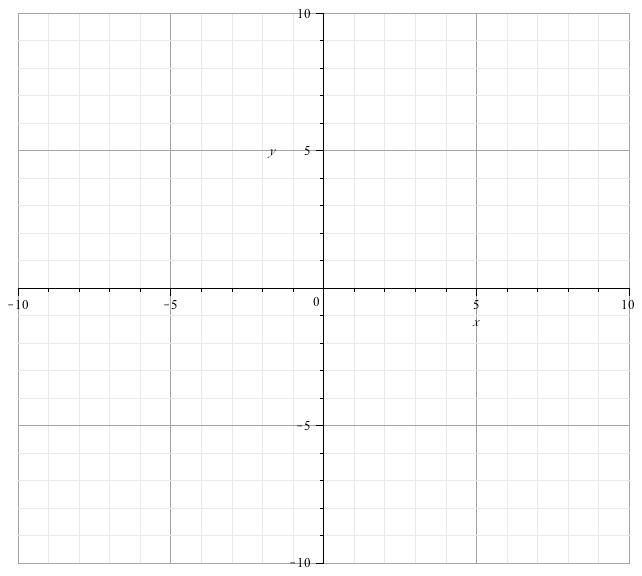
\includegraphics[scale=0.5]{graphpaper.jpg}
    \end{center}
  \end{enumerate}
\end{thm}

\newpage


\begin{thm}[10 Points]
  A box with a square base and open top must have a volume of \(32\ \text{cm}^3\).
  Find the dimensions of the box that minimize the amount of material used.\\
\end{thm}

\vspace{3in}

\begin{thm}[10 Points]
  Let
  \[f(x) = \int_0^x \cos(t)\dif t.\]
  Use Part I of the Fundamental Theorem of Calculus to evaluate
  \[\frac{\dif}{\dif x} f(x^2) = \frac{\dif}{\dif x} \int_0^{x^2} \cos(t)\dif t.\]

\end{thm}

\newpage

\begin{thm}[10 Points]\label{defn}
  Evaluate the integral \(\displaystyle{\int_0^2 3x^2 \dif x}\) using the limit definition of the integral and the identity
  \[\sum_{i = 1}^n i^2 = \frac{n(n+1)(2n + 1)}{6} = \frac{2n^3 + 3n^2 + n}{6}.\]
\end{thm}

\vspace{5in}

\begin{thm}[10 Points]
  Use the Fundamental Theorem of Calculus Part II to check your answer to Problem~\ref{defn}.
\end{thm}

\newpage

\begin{thm}[10 Points]
  Evaluate the indefinite integral
  \[\int\frac{\sin(x)}{\cos^2(x)}\dif x.\]
\end{thm}

\vspace{3in}

\begin{thm}[10 Points]
  Evaluate the indefinite integral
  \[\int \csc(\theta)\left(\sin(\theta) - \csc(\theta)\right)\dif \theta\]
\end{thm}

\newpage

\begin{thm}[10 Points]
  Evaluate the indefinite integral
  \[\int 2x\sqrt{x - 5}\dif x\]
\end{thm}

\vspace{3in}

\begin{thm}[10 Points]
  Evaluate the definite integral
  \[\int_0^{\sqrt{\pi}} x\sin(x^2)\dif x\]
\end{thm}

\newpage

\begin{thm}[10 Points]
  Given \(f^\prime(x) = 12x^2 + 6x - 4\) and \(f(1) = 1\), find \(f(x)\).
\end{thm}

\vspace{3in}

\begin{thm}[10 Points]
  Assume that \(f\) is an even function.
  Given
  \[\int_{-1}^3 f(x)\dif x = 3\ \text{and}\ \int_1^{3} f(x)\dif x = 1\]
  find
  \[\int_0^{1} f(x)\dif x.\]
\end{thm}
\end{document}
